% Template created by Karol Kozioł (www.karol-koziol.net) for ShareLaTeX

\documentclass[a4paper,9pt]{extarticle}
\usepackage[utf8]{inputenc}
\usepackage[T1]{fontenc}
\usepackage{graphicx}
\usepackage{xcolor}
\usepackage{tikz}

\usepackage{amsmath,amssymb,textcomp}
\everymath{\displaystyle}

\usepackage{times}
\renewcommand\familydefault{\sfdefault}
\usepackage{tgheros}
\usepackage[defaultmono,scale=0.85]{droidmono}

\usepackage{multicol}
\setlength{\columnseprule}{0pt}
\setlength{\columnsep}{20.0pt}


\usepackage{geometry}
\geometry{
a4paper,
total={210mm,297mm},
left=10mm,right=10mm,top=10mm,bottom=15mm}

\linespread{1.3}


% custom title
\makeatletter
\renewcommand*{\maketitle}{%
\noindent
\begin{minipage}{0.4\textwidth}

\begin{tikzpicture}
\node[rectangle,rounded corners=6pt,inner sep=10pt,fill=blue!50!black,text width= 0.95\textwidth] {\color{white}\Huge \@title};
\end{tikzpicture}
\end{minipage}
\hfill
\begin{minipage}{0.55\textwidth}
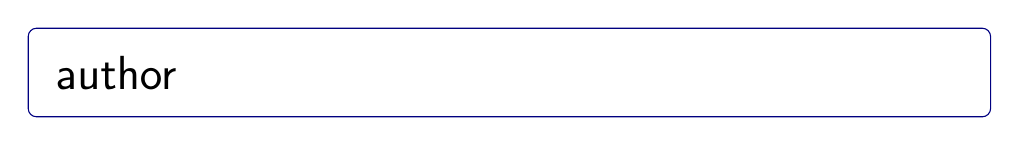
\begin{tikzpicture}
\node[rectangle,rounded corners=3pt,inner sep=10pt,draw=blue!50!black,text width= 0.95\textwidth] {\LARGE \@author};
\end{tikzpicture}
\end{minipage}
\bigskip\bigskip
}%
\makeatother

% custom section
\usepackage[explicit]{titlesec}
\newcommand*\sectionlabel{}
\titleformat{\section}
  {\gdef\sectionlabel{}
   \normalfont\sffamily\Large\bfseries\scshape}
  {\gdef\sectionlabel{\thesection\ }}{0pt}
  {
\noindent
\begin{tikzpicture}
\node[rectangle,rounded corners=3pt,inner sep=4pt,fill=blue!50!black,text width= 0.95\columnwidth] {\color{white}\sectionlabel#1};
\end{tikzpicture}
  }
\titlespacing*{\section}{0pt}{15pt}{10pt}


% custom footer
\usepackage{fancyhdr}
\makeatletter
\pagestyle{fancy}
\fancyhead{}
\fancyfoot[C]{\footnotesize \textcopyright\ \@date\ \ \@author}
\renewcommand{\headrulewidth}{0pt}
\renewcommand{\footrulewidth}{0pt}
\makeatother


\title{Math cheat sheet\ \ No.\ 123}
\author{Share\LaTeX\ or Some University or Something or even Something Else}
\date{2014}



\begin{document}

\maketitle

\begin{multicols*}{2}


\section{Algebra}

Lorem ipsum dolor sit amet, consectetur adipiscing elit, sed do eiusmod tempor incididunt ut labore et dolore magna aliqua. Ut enim ad minim veniam, quis nostrud exercitation ullamco laboris nisi ut aliquip ex ea commodo consequat. Duis aute irure dolor in reprehenderit in voluptate velit esse cillum dolore eu fugiat nulla pariatur. Excepteur sint occaecat cupidatat non proident, sunt in culpa qui officia deserunt mollit anim id est laborum.

\begin{tabular}{lll}
$a^n a^m = a^{n+m}$ & $\frac{a^n}{a^m} = a^{n-m}$ & $(a^n)^m = a^{n \cdot m}$\\
$a^n a^m = a^{n+m}$ & $\frac{a^n}{a^m} = a^{n-m}$ & $(a^n)^m = a^{n \cdot m}$\\
$a^n a^m = a^{n+m}$ & $\frac{a^n}{a^m} = a^{n-m}$ & $(a^n)^m = a^{n \cdot m}$\\
$a^n a^m = a^{n+m}$ & $\frac{a^n}{a^m} = a^{n-m}$ & $(a^n)^m = a^{n \cdot m}$\\
$a^n a^m = a^{n+m}$ & $\frac{a^n}{a^m} = a^{n-m}$ & $(a^n)^m = a^{n \cdot m}$\\
$a^n a^m = a^{n+m}$ & $\frac{a^n}{a^m} = a^{n-m}$ & $(a^n)^m = a^{n \cdot m}$
\end{tabular}


\section{Trigonometry}

Lorem ipsum dolor sit amet, consectetur adipiscing elit, sed do eiusmod tempor incididunt ut labore et dolore magna aliqua. 

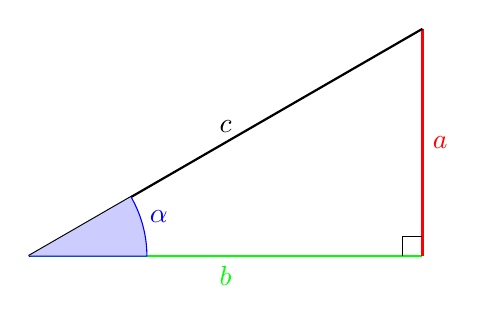
\begin{tikzpicture}[scale=5]
\draw[thick,color=green] (0,0) -- node[below] {$b$} (1,0);
\draw[thick,color=red] (1,0) -- node[right] {$a$} (1,0.57735);
\draw[thick,color=black] (1,0.57735) -- node[above] {$c$} (0,0);
\filldraw[fill=blue!20!white,draw=blue] (0,0) -- (0.3,0) arc (0:30:0.3); 
\node[color=blue] at (0.33,0.1) {$\alpha$};
\draw (0.95,0) -- (0.95,0.05) -- (1,0.05);
\end{tikzpicture}

\medskip

\begin{tabular}{ll}
$\sin\alpha = \frac{a}{c}$ & $\cos\alpha = \frac{b}{c}$ \\[1ex]
$\tan\alpha = \frac{a}{b}$ & $\cot\alpha = \frac{b}{a}$ \\
\end{tabular}

\section{Algebra (some very very very very very long title)}

\begin{tabular}{lll}
$a^n a^m = a^{n+m}$ & $\frac{a^n}{a^m} = a^{n-m}$ & $(a^n)^m = a^{n \cdot m}$\\
$a^n a^m = a^{n+m}$ & $\frac{a^n}{a^m} = a^{n-m}$ & $(a^n)^m = a^{n \cdot m}$\\
$a^n a^m = a^{n+m}$ & $\frac{a^n}{a^m} = a^{n-m}$ & $(a^n)^m = a^{n \cdot m}$\\
$a^n a^m = a^{n+m}$ & $\frac{a^n}{a^m} = a^{n-m}$ & $(a^n)^m = a^{n \cdot m}$\\
$a^n a^m = a^{n+m}$ & $\frac{a^n}{a^m} = a^{n-m}$ & $(a^n)^m = a^{n \cdot m}$\\
$a^n a^m = a^{n+m}$ & $\frac{a^n}{a^m} = a^{n-m}$ & $(a^n)^m = a^{n \cdot m}$
\end{tabular}


\section{Trigonometry}

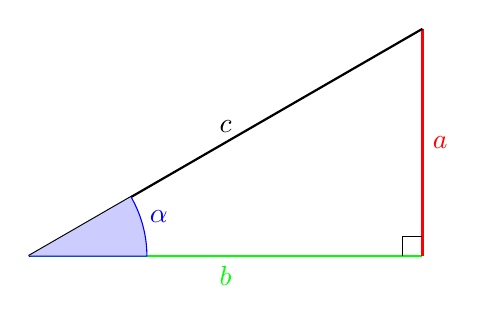
\begin{tikzpicture}[scale=5]
\draw[thick,color=green] (0,0) -- node[below] {$b$} (1,0);
\draw[thick,color=red] (1,0) -- node[right] {$a$} (1,0.57735);
\draw[thick,color=black] (1,0.57735) -- node[above] {$c$} (0,0);
\filldraw[fill=blue!20!white,draw=blue] (0,0) -- (0.3,0) arc (0:30:0.3); 
\node[color=blue] at (0.33,0.1) {$\alpha$};
\draw (0.95,0) -- (0.95,0.05) -- (1,0.05);
\end{tikzpicture}

\medskip

\begin{tabular}{ll}
$\sin\alpha = \frac{a}{c}$ & $\cos\alpha = \frac{b}{c}$ \\[1ex]
$\tan\alpha = \frac{a}{b}$ & $\cot\alpha = \frac{b}{a}$ \\
\end{tabular}


\section{Algebra}

\begin{tabular}{lll}
$a^n a^m = a^{n+m}$ & $\frac{a^n}{a^m} = a^{n-m}$ & $(a^n)^m = a^{n \cdot m}$\\
$a^n a^m = a^{n+m}$ & $\frac{a^n}{a^m} = a^{n-m}$ & $(a^n)^m = a^{n \cdot m}$\\
$a^n a^m = a^{n+m}$ & $\frac{a^n}{a^m} = a^{n-m}$ & $(a^n)^m = a^{n \cdot m}$\\
$a^n a^m = a^{n+m}$ & $\frac{a^n}{a^m} = a^{n-m}$ & $(a^n)^m = a^{n \cdot m}$\\
$a^n a^m = a^{n+m}$ & $\frac{a^n}{a^m} = a^{n-m}$ & $(a^n)^m = a^{n \cdot m}$\\
$a^n a^m = a^{n+m}$ & $\frac{a^n}{a^m} = a^{n-m}$ & $(a^n)^m = a^{n \cdot m}$
\end{tabular}


\section{Trigonometry}

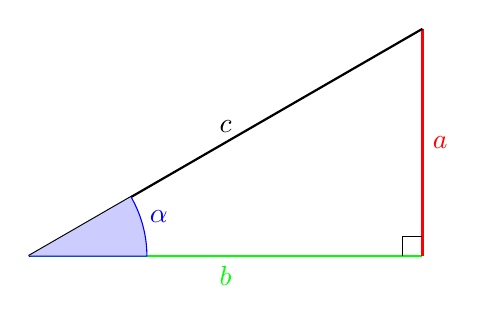
\begin{tikzpicture}[scale=5]
\draw[thick,color=green] (0,0) -- node[below] {$b$} (1,0);
\draw[thick,color=red] (1,0) -- node[right] {$a$} (1,0.57735);
\draw[thick,color=black] (1,0.57735) -- node[above] {$c$} (0,0);
\filldraw[fill=blue!20!white,draw=blue] (0,0) -- (0.3,0) arc (0:30:0.3); 
\node[color=blue] at (0.33,0.1) {$\alpha$};
\draw (0.95,0) -- (0.95,0.05) -- (1,0.05);
\end{tikzpicture}

\medskip

\begin{tabular}{ll}
$\sin\alpha = \frac{a}{c}$ & $\cos\alpha = \frac{b}{c}$ \\[1ex]
$\tan\alpha = \frac{a}{b}$ & $\cot\alpha = \frac{b}{a}$ \\
\end{tabular}


\section{The End}

Lorem ipsum dolor sit amet, consectetur adipiscing elit, sed do eiusmod tempor incididunt ut labore et dolore magna aliqua. Ut enim ad minim veniam, quis nostrud exercitation ullamco laboris nisi ut aliquip ex ea commodo consequat. Duis aute irure dolor in reprehenderit in voluptate velit esse cillum dolore eu fugiat nulla pariatur. Excepteur sint occaecat cupidatat non proident, sunt in culpa qui officia deserunt mollit anim id est laborum.


\end{multicols*}

\end{document}

